\section{Integrating Understandability into Retrieval}
\label{sec:experiments}

Next, we investigate how understandability estimations could be used and integrated into retrieval methods to increase the quality of search result. 
%
%We investigate here two real-world scenarios depending on the control a developer/researcher has over their system: 
%\begin{itemize}
%    \item Partial control: the developer/researcher is running a retrieval system which retrieves a ranked list of documents (not necessarily the score of each document) for a user query. 
%    \item Total control: the developer/researcher is an Information Retrieval expert and can implement/use a learning to rank system.
%\end{itemize}
%
%
%To achieve this, we applied selected understandability estimation approaches to improve the results of the selected retrieval runs. 

We introduce, as our first approach, a simple and effective method to explicitly increase understandability based on any understandability estimator. 
Given a pre-defined cut-off parameter, our approach blindly sorts the top retrieved documents up to this cut-off based on the understandability estimator.
With the job of retrieving topically relevant documents is left to the underline search engine, our approach focus on retrieving understandable documents.

An advantage of this approach is that it can be applied to any ranked list.
We evaluated the best readability formula for 2016 collection (Dale Chall, Table~\ref{tab:top_corr_metrics}) and several machine learning methods trained on top of a subset (or all) estimators listed in Table~\ref{tab:doc_features}. We model the machine learning experiments here as a regression task, which uses as training data the labels of documents assessed in CLEF 2016.
We predict scores for documents in the training set with a 10-fold cross validation and predict scores for documents outside the training set using all available data.

Our hypothesis is that such re-rank based solely on a understandability score is able to increase the understandability of the results ($P_u@10$) at the expenses of topical relevance ($P_r@10$). The understandability-relevance trade-off is primarily controlled by the cut-off. A relatively large cut-off, fifty, for instance, would allow the re-rank method to move a document from the 5th resulting page (considering the default 10 results per page) to the first one depending on the understandability score assigned to that document. We experiment with cut-offs at 15, 20 and 50 documents. 

Estimating a good cut-off parameter might be costly for a real world application...Alternatively to the cut-off control, we propose to automatically fuse the results of the relevance-optimized-system and the understandability-optimized-system into a single fused one.
This merge aims to retain the best of both extremes into a single system. For this, we used the Reciprocal Rank Fusion (RRF) method~\cite{cormack09}, which effectively combines two lists of search results based on the position of the results in a ranking.

Our second approach investigates how to blend understandability and relevance in a single step with learning to rank.

\todo{--- Stopped Here ---}

In the LTR we need to mention the combination of labels to make up the final document label which will be used by the method. Also, we need to say which method we used (pairwise tree boosting) and which are the features for each run....


In our experiments, we selected the top two systems at CLEF 2016 (based on their performance on $P@10$ \todo{check if they are the best systems for uRBP as well. It is likely.}) 
and created a plain BM25 system using the Terrier toolkit~\cite{terrier}. While we do not have access to the implementation of the first two systems, we have completely control over this BM25 system which will be useful later in our experiments.



%We explored both estimations based on readability formulas (we used Dale-Chall) and on machine learning regressors (we used linear regression). 
%These methods were used for re-ranking the top 20 search results returned by the initial systems. 

In the following we report results for CLEF 2016. Results for CLEF 2015 are included in the online appendix: they show similar trends to the 2016 results.

%Our experiments are based on the data collected during the Information Retrieval branch of CLEF eHealth. To the best of our knowledge that was the only venue in which topical and understandability assessments were collected. 
%We show here experiments with the CLEF eHealth 2016 campaign leaving 2015 experiments offline\footnote{Link to experiments will be available upon acceptance of this manuscript}.
%
%We start by the defining the evaluation measure that we will use here. 
%In CLEF eHealth campaign, organizers used a modification of RBP which ties together document relevance any other relevance dimension, in this case in particular, understandability \cite{clef16}.
%Mathematically, it consists in adding an understandability factor to the RBP formula: $uRBP(\rho) = (1 - \rho) \sum_{k=1}^{K} \rho^{K-1} r(d@K) u(d@k)$, with r(d@k) representing the gain in retrieving a topically relevant documents at rank $k$ and u(d@k) the gains coming from the understandability factor of a document at rank $k$.
%
%The drawback of such evaluation metric is that we cannot separately evaluate each dimension. We propose, instead, to separately evaluate a ranking list with respect to its topical relevance and its understandability:
%\begin{itemize}
%        \item $P_r@10$: a document is topically relevant if assessed as somewhat relevant or highly relevant. This metric counts the number of topically relevant documents in the top 10 documents of a ranked list.
%        \item $P_u@10$: a document is relevant for this metric if the understandability score is smaller than a threshold $U$. Like $P_r@10$, we count the number of relevant documents in the first 10 documents of a ranked list. We use $U = 40$ in our experiments. \todo{I decided to use this threshold based on the data. I will need to add a figure to support this clam, I think.}
%\end{itemize}
%
%During the campaign, organizers opt to use shallow pools and focus on highly ranked documents, using $P_r@10$ as one official metric for topical relevance.
%It makes our choice of metric natural. Likewise it is traditionally done with F measure, we combine $P_r@10$ and $P_u@10$ with an harmonic mean: $F_{ru} = 2 \times \frac{P_r@10 \times P_u@10}{P_r@10 + P_u@10}$. 
%
%When reranking runs, we risk to bring to the top of the rankings documents that were not assessed when the task took place. For this reason, we inform the average percentage of documents that were not assessed in the top 10 documents of each run (Unj@10) and we inform $P_r@10*$, $P_u@10*$ and $F_{ru}*$, modified measures that excluding all unassessed documents for the ranking list before evaluation.
%These last three metrics showcase the potential of a run if it had been included in the pool set.


% MOVE TO ONLINE APPENDIX:
%%%\begin{figure}
%%%    \caption{\todo{Feature selection experiment: different ML models were evaluated with various number of features in a 10 Cross Validation experiment. Top feature selection were made with mutual info algo. With 10 features, the selection made in our table 3 worked better than the selection automatically made mutual info. However, a larger number of features, at least 200, reached the best results. That explains why our L2R method worked better using all features than using only the selected set of 10 top features. We can discuss it in the text and link a better version of this figure in the online page. THe experiments made here can be improved if I run everything with XGB instead of LR. I am planning to do it tomorrow when I wake up.}}
%%%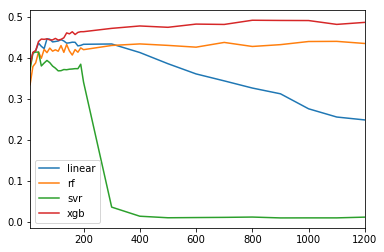
\includegraphics[width=0.3\textwidth]{graphics/features}
%%%\end{figure}


We start our experiments by showing at the top of Table~\ref{tab:experiments} (indices 1-3) the performance of the top 3 systems in CLEF eHealth 2016 together with a straightforward BM25 baseline run made with Terrier toolkit. Our further experiments will use not only these runs as a comparison base, but modify these runs when necessary.

The first batch of experiments, indices 4-6, consists of re-ranking the top 20 documents based solely on the Dale-Chall index, as it was the metrics with highest correlation with human judgements for this collection.
The topical relevance of the re-ranked resulting lists is immediately hurt in benefit of understandability. Note how $P_r@10$ and $P_r@10^*$ decrease while $P_u@10$ and in special $P_u@10^*$ increase.
The percentage of unassessed documents reach 10\% and, unfortunately, only looking at RBP and uRBP we cannot see the understandability benefits brought by the re-rank method.

The next batch of experiments swaps the Dale-Chall Index by a tree boosting method (aka. XGB or GBDT or GBM) learned using all features of Table~\ref{tab:doc_features}\footnote{Experiments with various Machine Learning methods and feature selection schemes were performed as well and are available in the online appendix. The results of other methods are similar. When using the set of top 10 features for each group from Table~\ref{tab:top_corr_metrics} results are always better than using an automatic method such as Chi Square to select 10 features to use.}.
While the higher correlation of Dale-Chall was XXX (as reported in table Y), correlations using XGB reached YYY, the closest method to the human agreement in this task.

Indices 7-15:
We experiment with reranking the top 15 (more more conservative method), 20 and 50 (a more heterodox method). We clearly see the trade-off between understandability and relevance when we increase from top 15 to top 50: while the $P_r@10$ falls 5 points, $P_u@10$ increases 10. Nevertheless, $F_{ru}*$ shows that more conservative methods provide the best trade-offs.
When comparing the use of Dale-Chall and Linear Regression reranking the same number of documents (indices 13-16), we notice that LR results for $P_u@10*$ are always superior to Dale-Chall, meaning it does a better job when bringing the easier documents to the top of the rank, but that not necessarily means the final rank is better, as we can see comparing the results for $F_{ru}*$.

Our third batch of experiments, indices 20-31, aims to combine the good ranking for topicality coming from the original rank list with the best rankings for understandability, coming from the LR reranking.
For that, we use the Reciprocal Rank Fusion (RRF) method, which combines runs on the rank of documents instead of scores~\cite{cormack09}. Reranking with LR and combining runs with RRF allows to obtain the best trade-offs so far, with $F_{ru}$ of the best method in CLEF being improved from 39.05 to 39.68, with comes from a very small decrease in $P_u@10*$ (from 31.70 to 31.60) and a 4.9\% increase in $P_u@10*$ (from 50.83 to 53.30).

Our final batch of experiments, indices 32-34, are based on learning-to-rank. We decided to use the pairwise implementation of the gradient boosting approach from the XGBoost framework~\cite{chen16} due to its recent good results in many machine learning tasks \todo{actually, I should use XGBoost method instead of LR}. Evaluating other learning to rank methods and frameworks are left as future work.
We evaluated three different settings based on the plain BM25 run shown in index 4, each one with a different combination of feature set and relevance labels:
\begin{itemize}
    \item Index 32: we used as relevance labels only the topical labels and as feature set the score of different information retrieval models (BM25, Dirichlet LM and PL2). This represents the typical use of learning to rank aiming to optimize only the topical relevance results. Unfortunately that was not the case and not even the $P_r@10*$ was improved.
    \item Index 33: we used as relevance labels the linear combination of topical relevance and understandability. Additionally to the IR features, we used the 10 features correspondent to the best features according to Kendall tau in Table~\ref{tab:top_corr_metrics}. Results show that this resulted in higher $F_{ur}*$ when compared to its correspondent approaches (indices 4, 8, 12, 16, 19, 23, 27 and 31) due to a high increase in $P_r@10*$, which reveals understandability features improving topicability.
    \item Index 34: On top of our previous run, we included here all features shown in Table~\ref{tab:doc_features}. Note that despite the very high number of unassessed documents, this run shows improvements even in $P_r@10$ obtaining the same results as the third best run in the campaign (ECNU). In its turn, the $P_{r}*$ which ignores the unassessed documents is 8.4\% higher than the best system, while $F_{ru}*$ is 5.2\% higher.
\end{itemize}


\begin{table*}[ht!]
\caption{Results obtained by integrating understandability estimations within
retrieval methods on CLEF 2016. Baseline runs are reported at table
indices 1-3. Re-ranking experiments are reported at indices 4-21.
Fusion experiments are reported at indices 22-30. Learning to rank
experiments are reported at indices 31-35. All measures were calculated
up to rank $n=10$. }
%\vspace{-0.2cm}
 \label{tab:experiments} 
\resizebox{1.00\textwidth}{!}{ %
\begin{tabular}{cclllllllllllll}
\toprule 
    \multirow{2}{*}{Index }  & \multirow{2}{*}{Rerank }  & \multirow{2}{*}{Run }  & \multicolumn{4}{l}{Official CLEF 2016 Metrics} & \multicolumn{8}{l}{New Metrics to Evaluate Underst. in Retrieval - Sec.~\ref{sec:data}}\tabularnewline
\cmidrule(l{2pt}r{2pt}){4-7} \cmidrule(l{2pt}r{2pt}){8-15}  &  &  & $RBP$  & RBP Res.  & uRBP  & uRBP Res.  & $RBP_{u}$  & $RBP_{u}$ Res. & $HRBP$  & HRBP Res. & Unj  & $RBP_{r}^{*}$  & $RBP_{u}^{*}$  & $HRBP^{*}$\tabularnewline
\midrule 
1  & \multirow{3}{*}{No Rerank}  & GUIR~\cite{soldaini16} (Best Run)  & \textbf{28.11}  & 7.65  & \textbf{18.12}  & 7.19  & \textbf{45.69}  & 8.86 & \textbf{25.61}  & 6.50 & 0.01  & \textbf{28.29}  & \textbf{46.03}  & \textbf{25.79} \tabularnewline
2  &  & ECNU~\cite{song16} (Runner Up)  & 27.70  & 7.37  & 17.55  & \textbf{7.34}  & 43.89$^{\diamond}$  & 8.66 & 25.35  & 6.26 & 0.01  & 27.77  & 44.18$^{\diamond}$  & 25.48 \tabularnewline
3  &  & Plain BM25 Baseline  & 25.28$^{\diamond}$  & \textbf{8.24}  & 16.05$^{\diamond}$  & 6.94  & 42.08$^{\diamond}$  & \textbf{10.97} & 22.97$^{\diamond}$  & \textbf{7.19} & \textbf{0.06}  & {26.01}$^{\diamond}$  & {43.89}$^{\diamond}$  & {23.93}$^{\diamond}$ \tabularnewline
\midrule 
4  & \multirow{3}{*}{\makecell{Dale-Chall Top 15}}  & Based on GUIR  & 24.70$^{\dagger\diamond}$  & 8.70  & 16.83$^{\dagger\diamond}$  & 7.27  & 49.10$^{\dagger\diamond}$  & 10.62 & 24.94  & 7.50 & 0.03  & 25.24$^{\dagger\diamond}$  & 50.33$^{\dagger\diamond}$  & 25.54 \tabularnewline
5  &  & Based on ECNU  & 24.78$^{\dagger\diamond}$  & 7.83  & 16.64$^{\diamond}$  & 7.16  & 48.88$^{\dagger\diamond}$  & 9.71 & 24.80  & 6.50 & 0.02  & 25.12$^{\dagger\diamond}$  & 49.64$^{\dagger\diamond}$  & 25.21 \tabularnewline
6  &  & Based on BM25  & 23.22$^{\dagger\diamond}$  & 8.78  & 15.85 $^{\diamond}$  & 6.94  & 47.09$^{\dagger\diamond}$  & 11.83 & 24.01  & 7.42 & 0.07  & 24.04$^{\dagger\diamond}$  & 48.60$^{\dagger\diamond}$  & 24.82 \tabularnewline
\hdashline 7  & \multirow{3}{*}{\makecell{Dale-Chall Top 20}}  & Based on GUIR  & 22.19$^{\dagger\diamond}$  & 9.37  & 15.36$^{\dagger\diamond}$  & 6.98  & 48.71$^{\dagger\diamond}$  & 12.30 & 23.21$^{\dagger\diamond}$  & 8.12 & 0.06  & 23.26$^{\dagger\diamond}$  & 51.39$^{\dagger\diamond}$  & 24.45$^{\dagger\diamond}$\tabularnewline
8  &  & Based on ECNU  & 23.01$^{\dagger\diamond}$  & 8.93  & 15.70$^{\dagger\diamond}$  & 6.91  & 48.99$^{\dagger\diamond}$  & 11.69 & 23.73$^{\dagger\diamond}$  & 7.80 & 0.05  & 23.84$^{\dagger\diamond}$  & 51.00$^{\dagger\diamond}$  & 24.66\tabularnewline
9  &  & Based on BM25  & 21.58$^{\dagger\diamond}$  & 9.51  & 14.83$^{\dagger\diamond}$  & 7.02  & 46.99$^{\dagger}$  & 13.00 & 22.89$^{\diamond}$  & 8.06 & 0.09  & 22.93$^{\dagger\diamond}$  & 49.55$^{\dagger\diamond}$  & 24.26\tabularnewline
\hdashline 10  & \multirow{3}{*}{\makecell{Dale-Chall Top 50}}  & Based on GUIR  & 16.18$^{\dagger\diamond}$  & 15.24  & 11.56$^{\dagger\diamond}$  & 6.80  & 41.79$^{\dagger\diamond}$  & 24.49 & 18.10$^{\dagger\diamond}$  & 14.42 & 0.22  & 20.90$^{\dagger\diamond}$  & 53.28$^{\dagger\diamond}$  & 23.27$^{\dagger\diamond}$ \tabularnewline
11  &  & Based on ECNU  & 16.88$^{\dagger\diamond}$  & 17.37  & 11.78$^{\dagger\diamond}$  & \textbf{7.30}  & 40.76$^{\dagger\diamond}$  & 23.77 & 18.30$^{\dagger\diamond}$  & \textbf{15.57} & \textbf{0.24}  & 21.34$^{\dagger\diamond}$  & 52.07$^{\dagger\diamond}$  & 23.33$^{\dagger\diamond}$ \tabularnewline
12  &  & Based on BM25  & 15.06$^{\dagger\diamond}$  & 15.35$^{\dagger\diamond}$  & 10.55  & 6.62  & 40.03 $^{\diamond}$  & 23.88 & 16.55$^{\dagger\diamond}$  & 13.83 & \textbf{0.24}  & 19.42$^{\dagger\diamond}$  & 51.69$^{\dagger\diamond}$  & 21.59$^{\dagger\diamond}$ \tabularnewline
\hdashline 13  & \multirow{3}{*}{\makecell{XGB Top 15}}  & Based on GUIR  & \textbf{25.16}$^{\dagger\diamond}$  & 8.09  & \textbf{17.27}$^{\dagger\diamond}$  & 7.12  & \textbf{50.96}$^{\dagger\diamond}$  & 10.11 & \textbf{25.16}  & 6.89 & 0.02  & \textbf{25.61}$^{\dagger\diamond}$  & 52.00$^{\dagger\diamond}$  & \textbf{25.68}\tabularnewline
14  &  & Based on ECNU  & 24.18$^{\dagger\diamond}$  & 7.69  & 16.54 $^{\diamond}$  & 7.09  & 50.00$^{\dagger\diamond}$  & 9.91 & 24.56  & 6.65 & 0.02  & 24.56$^{\dagger\diamond}$  & 50.74$^{\dagger\diamond}$  & 25.01\tabularnewline
15  &  & Based on BM25  & 22.33$^{\dagger\diamond}$  & 8.14  & 15.46  & 6.76  & 47.90$^{\dagger\diamond}$  & 12.13 & 22.89$^{\diamond}$  & 7.25 & 0.07  & 23.11$^{\dagger\diamond}$  & 49.43$^{\dagger\diamond}$  & 23.69$^{\diamond}$\tabularnewline
\hdashline 16  & \multirow{3}{*}{\makecell{XGB Top 20}}  & Based on GUIR  & 22.38$^{\dagger\diamond}$  & 9.49  & 15.61$^{\dagger\diamond}$  & 7.05  & 50.45$^{\dagger\diamond}$  & 12.08 & 23.30$^{\dagger\diamond}$  & 8.16 & 0.05  & 23.62$^{\dagger\diamond}$  & 52.98$^{\dagger\diamond}$  & 24.68\tabularnewline
17  &  & Based on ECNU  & 22.95$^{\dagger\diamond}$  & 8.82  & 15.95$^{\dagger\diamond}$  & 7.02  & 50.42$^{\dagger\diamond}$  & 11.70 & 23.97$^{\diamond}$  & 7.56 & 0.04  & 23.68$^{\dagger\diamond}$  & 52.15$^{\dagger\diamond}$  & 24.73\tabularnewline
18  &  & Based on BM25  & 20.65$^{\dagger\diamond}$  & 9.42  & 14.46$^{\dagger\diamond}$  & 6.84  & 47.74$^{\dagger\diamond}$  & 13.56 & 21.93$^{\diamond}$  & 8.34 & 0.09  & 21.98$^{\dagger\diamond}$  & 50.28$^{\dagger\diamond}$  & 23.27$^{\diamond}$\tabularnewline
\hdashline 19  & \multirow{3}{*}{\makecell{XGB Top 50}}  & Based on GUIR  & 16.65$^{\dagger\diamond}$  & 15.73  & 12.39$^{\dagger\diamond}$  & 6.84  & 43.49$^{\dagger\diamond}$  & 23.63 & 18.70$^{\dagger\diamond}$  & 13.74 & 0.22  & 21.13$^{\dagger\diamond}$  & \textbf{55.07}$^{\dagger\diamond}$  & 23.58$^{\dagger\diamond}$\tabularnewline
20  &  & Based on ECNU  & 16.19$^{\dagger\diamond}$  & \textbf{17.01}  & 11.82$^{\dagger\diamond}$  & 7.27  & 43.05$^{\diamond}$  & \textbf{24.75} & 18.27$^{\dagger\diamond}$  & 14.41 & \textbf{0.24}  & 20.16$^{\dagger\diamond}$  & 54.70$^{\dagger\diamond}$  & 22.96$^{\dagger\diamond}$\tabularnewline
21  &  & Based on BM25  & 15.43$^{\dagger\diamond}$  & 15.37  & 11.33$^{\dagger\diamond}$  & 6.48  & 41.93$^{\diamond}$  & 23.65 & 17.43$^{\dagger\diamond}$  & 13.40 & 0.26  & 19.58$^{\dagger\diamond}$  & 54.04$^{\dagger\diamond}$  & 22.17$^{\dagger\diamond}$\tabularnewline
\midrule 
22  & \multirow{3}{*}{\makecell{RRF (XGB \& Orig.) Top 15} }  & Based on GUIR  & \textbf{27.23}$^{\dagger\diamond}$  & 7.76  & \textbf{18.31}  & \textbf{7.23}  & 49.69$^{\dagger\diamond}$  & 9.18 & 26.49$^{\dagger\diamond}$  & 6.62 & 0.01  & \textbf{27.46}$^{\dagger\diamond}$  & 50.07$^{\dagger\diamond}$  & \textbf{26.69}$^{\dagger\diamond}$\tabularnewline
23  &  & Based on ECNU  & 26.60$^{\dagger\diamond}$  & 7.41  & 17.81  & 7.19  & 48.67$^{\dagger\diamond}$  & 8.80 & 26.02  & 6.09 & 0.01  & 26.76$^{\dagger\diamond}$  & 49.10$^{\dagger\diamond}$  & 26.27$^{\dagger}$ \tabularnewline
24  &  & Based on BM25  & 24.57$^{\diamond}$  & 8.15  & 16.51$^{\diamond}$  & 6.91  & 46.76$^{\dagger}$  & 11.23 & 24.16$^{\dagger}$  & 7.20 & 0.06  & 25.32$^{\diamond}$  & 48.52$^{\dagger\diamond}$  & 25.08$^{\dagger}$ \tabularnewline
\hdashline 25  & \multirow{3}{*}{\makecell{RRF (XGB \& Orig.) Top 20}}  & Based on GUIR  & 26.21$^{\dagger\diamond}$  & 7.96  & 17.73  & 7.19  & 50.29$^{\dagger\diamond}$  & 9.58 & 25.89  & 6.73 & 0.03  & 26.53$^{\dagger\diamond}$  & 50.98$^{\dagger\diamond}$  & 26.25\tabularnewline
26  &  & Based on ECNU  & 26.15$^{\dagger\diamond}$  & 7.64  & 17.69  & 7.09  & 49.70$^{\dagger\diamond}$  & 9.28 & \textbf{26.07 } & 6.39 & 0.02  & 26.38$^{\dagger\diamond}$  & 50.32$^{\dagger\diamond}$  & 26.35\tabularnewline
27  &  & Based on BM25  & 24.04$^{\dagger\diamond}$  & 8.24  & 16.32$^{\diamond}$  & 6.87  & 47.69$^{\dagger\diamond}$  & 11.40 & 24.08$^{\dagger\diamond}$  & 7.35 & 0.06  & 24.82$^{\dagger\diamond}$  & 49.52$^{\dagger\diamond}$  & 25.01$^{\dagger}$ \tabularnewline
\hdashline 28  & \multirow{3}{*}{\makecell{RRF (XGB \& Orig.) Top 50}}  & Based on GUIR  & 24.09$^{\dagger\diamond}$  & \textbf{9.44}  & 16.85$^{\dagger\diamond}$  & 7.02  & 50.55$^{\dagger\diamond}$  & 11.76 & 24.76  & \textbf{8.01} & 0.07  & 25.08$^{\dagger\diamond}$  & \textbf{52.84}$^{\dagger\diamond}$  & 25.84\tabularnewline
29  &  & Based on ECNU  & 24.17$^{\dagger\diamond}$  & 8.67  & 16.75$^{\diamond}$  & 7.12  & \textbf{50.63}$^{\dagger\diamond}$  & 11.66 & 25.00  & 7.61 & 0.07  & 24.90$^{\dagger\diamond}$  & 52.50$^{\dagger\diamond}$  & 25.84 \tabularnewline
30  &  & Based on BM25  & 22.28$^{\dagger\diamond}$  & 8.87 & 15.50  & 6.76  & 48.79$^{\dagger\diamond}$  & \textbf{12.90} & 23.13$^{\dagger\diamond}$  & 7.82 & \textbf{0.10 } & 23.46$^{\dagger\diamond}$  & 51.89$^{\dagger\diamond}$  & 24.57\tabularnewline
\midrule 
31  & \multirow{5}{*}{XGB LeToR}  & Combo 1 on BM25  & 20.42$^{\dagger\diamond}$  & 17.61  & 13.00$^{\dagger\diamond}$  & 7.41  & 32.17$^{\dagger\diamond}$  & 24.61 & 18.39$^{\dagger\diamond}$  & 14.41 & 0.28  & 25.25$^{\diamond}$  & 43.19$^{\diamond}$  & 23.83$^{\diamond}$\tabularnewline
32  &  & Combo 2 on BM25  & 24.98$^{\dagger\diamond}$  & 19.83  & 15.30$^{\dagger\diamond}$  & 8.09  & 35.09$^{\dagger\diamond}$  & 25.14 & 22.26$^{\diamond}$  & 17.50 & 0.24  & 30.41  & 46.09  & 28.28$^{\dagger\diamond}$ \tabularnewline
33  &  & Combo 3 on BM25  & 26.35$^{\dagger}$  & \textbf{20.48}  & 15.88$^{\dagger\diamond}$  & 8.16  & 34.73$^{\dagger\diamond}$  & 24.69 & 21.81$^{\dagger}$  & 17.41 & 0.22  & 32.25$^{\diamond}$  & 45.44  & 28.22$^{\dagger\diamond}$\tabularnewline
34  &  & Combo 4 on BM25  & 16.16$^{\dagger\diamond}$  & 19.48  & 10.76$^{\dagger\diamond}$  & 7.27  & \textbf{36.75}$^{\dagger\diamond}$  & \textbf{28.51} & 16.77$^{\dagger\diamond}$  & \textbf{17.80} & \textbf{0.29 } & 22.20$^{\dagger\diamond}$  & \textbf{50.06}$^{\dagger\diamond}$  & 23.32$^{\diamond}$\tabularnewline
35  &  & Combo 5 on BM25  & \textbf{26.76}$^{\diamond}$  & \textbf{20.48}  & \textbf{16.19}$^{\diamond}$  & \textbf{8.34}  & 35.26$^{\dagger\diamond}$  & 24.13 & \textbf{22.96}  & 17.59 & 0.22  & \textbf{32.60}$^{\dagger}$  & 45.87  & \textbf{29.20}$^{\dagger\diamond}$\tabularnewline
\bottomrule
\end{tabular}
} % end of resizebox
\end{table*}




